% Hlavicka pro protokoly z fyzikalniho praktika.
% Verze pro: LaTeX
% Verze hlavicky: 22. 2. 2007
% Autor: Ustav fyziky kondenzovanych latek
% Ke stazeni: www.physics.muni.cz/ufkl/Vyuka/
% Licence: volne k pouziti, nejlepe k vcasnemu odevzdani protokolu z Vaseho mereni.

\documentclass[a4paper,11pt]{article}

% Kodovani (cestiny) v dokumentu: utf-8
%\usepackage[cp1250]{inputenc}	% Omezena stredoevropska kodova stranka, pouze MSW.
\usepackage[utf8]{inputenc}	% Doporucujeme pouzivat UTF-8 (unicode).

%%% Nemente:
\usepackage[margin=2cm]{geometry}
\newtoks\jmenopraktika \newtoks\jmeno \newtoks\datum
\newtoks\obor \newtoks\skupina \newtoks\rocnik \newtoks\semestr
\newtoks\cisloulohy \newtoks\jmenoulohy
\newtoks\tlak \newtoks\teplota \newtoks\vlhkost
\usepackage{amsmath}
\usepackage{mathtools}
\usepackage{graphicx}
\usepackage{multirow}
\graphicspath{ {./images/} }
%%% Nemente - konec.


%%%%%%%%%%% Doplnte pozadovane polozky:

\jmenopraktika={Fyzikální praktikum 2}  % nahradte jmenem vaseho predmetu
\jmeno={Artem Gorodilov}            % nahradte jmenem mericiho
\datum={18. ~prosince  2023}        % nahradte datem mereni ulohy
\obor={Astrofyzika}                     % nahradte zkratkou vami studovaneho oboru
\skupina={Čt 8:00}            % nahradte dobou vyuky vasi seminarni skupiny
\rocnik={II}                  % nahradte rocnikem, ve kterem studujete
\semestr={I}                 % nahradte semestrem, ve kterem studujete

\cisloulohy={11}               % nahradte cislem merene ulohy
\jmenoulohy={Interference a difrakce světla} % nahradte jmenem merene ulohy

\tlak={986}                   % nahradte tlakem pri mereni (v hPa)
\teplota={20.9}               % nahradte teplotou pri mereni (ve stupnich Celsia)
\vlhkost={42}               % nahradte vlhkosti vzduchu pri mereni (v %)

%%%%%%%%%%% Konec pozadovanych polozek.


%%%%%%%%%%% Uzitecne balicky:
\usepackage[czech]{babel}
\usepackage{graphicx}
\usepackage{amsmath}
\usepackage{xspace}
\usepackage{url}
\usepackage{indentfirst}
\usepackage{listings}
\usepackage{subcaption}
\usepackage{caption}
\usepackage{tabularx}
\usepackage[labelformat=parens,labelsep=quad,skip=3pt]{caption}

%%%%%% Zamezeni parchantu:
\widowpenalty 10000 \clubpenalty 10000 \displaywidowpenalty 10000
%%%%%% Parametry pro moznost vsazeni vetsiho poctu obrazku na stranku
\setcounter{topnumber}{3}	  % max. pocet floatu nahore (specifikace t)
\setcounter{bottomnumber}{3}	  % max. pocet floatu dole (specifikace b)
\setcounter{totalnumber}{6}	  % max. pocet floatu na strance celkem
\renewcommand\topfraction{0.9}	  % max podil stranky pro floaty nahore
\renewcommand\bottomfraction{0.9} % max podil stranky pro floaty dole
\renewcommand\textfraction{0.1}	  % min podil stranky, ktery musi obsahovat text
\intextsep=8mm \textfloatsep=8mm  %\intextsep pro ulozeni [h] floatu a \textfloatsep pro [b] or [t]

% Tecky za cisly sekci:
\renewcommand{\thesection}{\arabic{section}.}
\renewcommand{\thesubsection}{\thesection\arabic{subsection}.}
% Jednopismenna mezera mezi cislem a nazvem kapitoly:
\makeatletter \def\@seccntformat#1{\csname the#1\endcsname\hspace{1ex}} \makeatother

\begin{document}

\thispagestyle{empty}

{
\begin{center}
\sf 
{\Large Ústav fyzikální elektroniky PřF MU} \\
\bigskip
{\huge \bfseries FYZIKÁLNÍ PRAKTIKUM} \\
\bigskip
{\Large \the\jmenopraktika}
\end{center}

\bigskip

\sf
\noindent
\setlength{\arrayrulewidth}{1pt}
\begin{tabular*}{\textwidth}{@{\extracolsep{\fill}} l l}
\large {\bfseries Zpracoval:}  \the\jmeno & \large  {\bfseries Naměřeno:} \the\datum\\[2mm]
\large  {\bfseries Obor:} \the\obor  \hspace{40mm}  {\bfseries Skupina:} \the\skupina %
%{\bfseries Ročník:} \the\rocnik \hspace{5mm} {\bfseries Semestr:} \the\semestr  
&\large {\bfseries Testováno:}\\
\\
\hline
\end{tabular*}
}

\bigskip

{
\sf
\noindent \begin{tabular}{p{3cm} p{0.6\textwidth}}
\Large  Úloha č. {\bfseries \the\cisloulohy:} \par
\smallskip
$T=\the\teplota$~$^\circ$C \par
$p=\the\tlak$~hPa \par
$\varphi=\the\vlhkost$~\%
&\Large \bfseries \the\jmenoulohy  \\[2mm]
\end{tabular}
}

\vskip1cm
    \begin{minipage}[t]{0.5\textwidth} 
        \section{Zadání}
            Určit tloušťku tenké vrstvy pomocí Michelsonova interferometru.
            \par Určit index lomu vzduchu pomocí Michelsonova interferometru. 
            \par Určit hustotu vrypů optické mřížky.
        \section{Teorie}
            \subsection{Tloušťka tenké vrstvy}
                K určení tloušťky tenké vrstvy použijeme Michelsonův interferometr. Má zelený laser s vlnovou délkou $\lambda$ = 531,2 nm. Tento interferometr promítá interferenční obrazec na stínítku.
                \par Když změníme sklon zrcadla interferometru, změníme fázový posun, čímž se změní interferenční obrazec. Toto měření je vyjádřeno různými hodnotami vzdálenosti dvou interferenčních paprsků $x_1$ a posunem interferenčních proužků $x_2$. Situaci lze vidět na obrázku (1).
                \par Z toho je možné vypočítat tloušťku tenké vrstvy podle vzorce:
                \begin{equation}
                    t = \frac{x_2}{x_1} \frac{\lambda}{2}
                \end{equation}
            \subsection{Index lomu vzduchu}
                \par Pro měření indexu lomu vzduchu budu vzduch z kyvety se vzorkem odčerpávat pomocí kompresoru.
                \par Poté kompresor vypnu a počkám, až se tlak vyrovná. Vzhledem ke změně indexu lomu $n$ v kyvetě se v důsledku rozdílu tlaků $\Delta p$ změní interferenční obrazec.
    \end{minipage}
    \hspace{10pt}
    \begin{minipage}[t]{0.5\textwidth} 
            \vspace{0pt}   
            \par \centering
            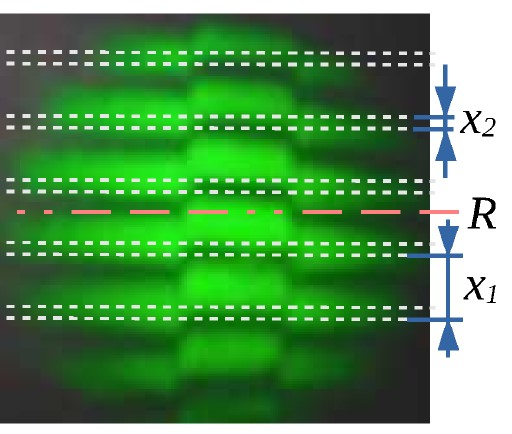
\includegraphics[scale=0.5]{inter}
            \captionsetup{justification=centering, font=footnotesize}
            \captionof{figure}{Vzdalenost dvou interferencnich paprsku $x_1$ a posun interferencnich pruzku $x_2$}
            \label{fig:inter}
            \vspace{10pt}
            \raggedright
            \par Nejprve se interferenční čáry posunou směrem nahoru, jak tlak klesá, a poté se posunou směrem dolů, jakmile se tlak vyrovná s atmosférickým tlakem $p_{vz}$.
            \par Odtud zjistíme index lomu vzduchu $n$ pomocí vzorce: 
            \begin{equation}
                n_{vz} = 1 + \frac{N \lambda}{2d} \frac{p_{vz}}{\Delta p}
            \end{equation}
            kde $N$ je počet interferenčních proužků, $\lambda$ je vlnová délka laseru a $d$ je délka kyvety.
            \par Rozdíl tlaků $\Delta p$ se bude rovnat:
            \begin{equation}
                \Delta p = p_{vz} - p_1
            \end{equation}
            kde $p_1$ je tlak pri odčerpávání vzduchu.
        \subsection{Hustota vrypů optické mřížky}
            Pro měření hustoty vtisku difrakční mřížky propusťme laser o vlnové délce $\lambda$ = 632.8 nm (červený). 
    \end{minipage}
\newpage
    \begin{minipage}[t]{0.5\textwidth}
            \par Na obrazovce se pak zobrazí difrakční obrazec. Situace je vidět na obrázku (2). Při znalosti poloh difrakčních maxim můžeme vzdálenosti jednotlivých vrypů na mřížce $d$ zjistit podle vzorce:
            \begin{equation}
                d = m\lambda \frac{\sqrt{y^2_m + x^2}}{y_m} ~~,~~ m = 1, 2, 3, ...
            \end{equation}
            kde $m$ je pořadí difrakčního maxima, $y_m$ je poloha difrakčního maxima a $x$ je vzdálenost do difrakčního obrazcu.
            \par Polohy difrakčních maxim $y_m$ jsou dány vztahem:
            \begin{equation}
                y_m = \frac{y_m'+y_m''}{2}
            \end{equation}
            kde $y_m'$ je poloha difrakčního maxima nalevo od středu difrakčního obrazce a $y_m''$ je poloha difrakčního maxima napravo od středu difrakčního obrazce.
            \par Pak hustotu vrypů optické mřížky $N$ můžeme zjistit podle vzorce:
            \begin{equation}
                N = \frac{1}{d}
            \end{equation}
            \vspace{10pt}   
            \par \centering
            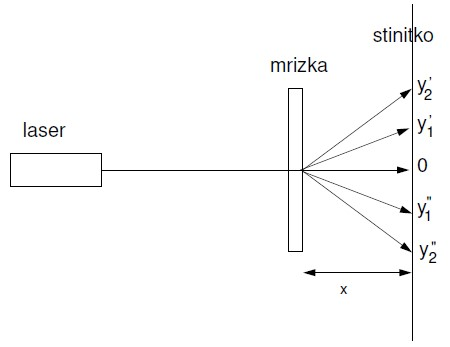
\includegraphics[scale=0.5]{dif}
            \captionsetup{justification=centering, font=footnotesize}
            \captionof{figure}{Schéma difrakční mřížky}
            \label{fig:dif}
            \vspace{10pt}
            \raggedright
    \section{Měření}  
        \subsection{Tloušťka tenké vrstvy}
            Pro měření tloušťky tenké vrstvy jsme změřili hodnoty $x_1$ a $x_2$ pro tři různé polohy zrcátka interferometru. Výsledky měření jsou uvedeny v tabulce (1).
        \end{minipage}
    \hspace{10pt}
    \begin{minipage}[t]{0.5\textwidth}  
            \par Poté jsme změřili tloušťku tenké vrstvy pro každý stav systému podle vzorce (1). Výsledky měření jsou uvedeny v tabulce (2).
            \vspace{10pt}
            \par \centering
            \begin{tabular}{|c|c|c|}
                \hline
                $t_1$ [nm] & $t_2$ [nm] & $t_3$ [nm] \\
                \hline
                65(3) & 66(3) & 68(3) \\
                \hline
                65(3) & 66(3) & 66(3) \\
                \hline
                64(4) & 66(3) & 66(3) \\
                \hline
                65(3) & 67(4) & 65(3) \\
                \hline
                64(3) & 65(3) & 69(3) \\
                \hline
                \end{tabular}
            \captionsetup{justification=centering, font=footnotesize}
            \captionof{table}{Vypočtené hodnoty tloušťky tenké vrstvy pro tři různé polohy zrcátka interferometru}
            \vspace{10pt}
            \raggedright
            \par Odtud získáme hodnotu tloušťky tenké vrstvy $t$:  
            \begin{center}
                $t$ = 66(2) nm
            \end{center}
        \subsection{Index lomu vzduchu}
            Po měření byly získány následující hodnoty $p_{vz}$, $\Delta p$, $d$ a $N$:
            \begin{center}
                $p_{vz}$ = 98600 Pa
                \vspace{5pt}
                \par $\Delta p$ = 0.73 $\frac{kg}{cm^2}$ = 71589 Pa
                \vspace{5pt}
                \par $d$ = 40 mm
                \vspace{5pt}
                \par $N$ = 23.0(5)
            \end{center}
            Odtud zjistíme hodnoty indexu lomu světla pro vzduch podle vzorce (2): 
            \begin{center}
                $n_{vz}$ = 1.000210(5)
            \end{center}
        \subsection{Hustota vrypů optické mřížky}
            Pro měření hustoty vrypů optické mřížky jsme změřili polohy difrakčních maxim $y_1'$, $y_1''$ a $y_2'$, $y_2''$ pro 4 různých stavů soustavy pro mřížku nominální hustotou vrypů 300 mm$^{-1}$ a 600 mm$^{-1}$ resp. 
            \par Hodnoty $y_1$ a $y_2$ pak byly vypočteny podle vzorce (5) a hodnoty $d$ pro každou z konfigurací systému byly vypočteny podle vzorce (4). Výsledky měření jsou uvedeny v tabulce (3) a (4).

    \end{minipage}
                \vspace{10pt}
                \par \centering
                \begin{tabular}{|c|c|c|c|c|c|}
                    \hline
                    \multicolumn{2}{|c}{poloha №1} & \multicolumn{2}{|c|}{poloha №2} &  \multicolumn{2}{c|}{poloha №3} \\
                    \hline
                    $x_{1,1}$ [px] & $x_{1,2}$ [px] & $x_{2,1}$ [px] & $x_{2,2}$ [px] & $x_{3,1}$ [px] & $x_{3,2}$ [px] \\
                    \hline
                    103(1) & 25(1) & 105(1) & 26(1) & 110(1) & 28(1) \\
                    \hline
                    86(1) & 21(1) & 93(1) & 23(1) & 101(1) & 25(1) \\
                    \hline
                    75(1) & 18(1) & 104(1) & 26(1) & 109(1) & 27(1) \\
                    \hline
                    102(1) & 25(1) & 75(1) & 19(1) & 86(1) & 21(1) \\
                    \hline
                    91(1) & 22(1) & 90(1) & 22(1) & 93(1) & 24(1) \\
                    \hline
                \end{tabular}
                \captionsetup{justification=centering, font=footnotesize}
                \captionof{table}{Naměřené hodnoty $x_1$ a $x_2$ pro tři různé polohy zrcátka interferometru}
                \vspace{0pt}
                \raggedright
\newpage
                \begin{table}[t]   
                    \centering
                    \begin{tabular}{|c|c|c|c|c|c|c|c|c|}
                        \hline
                        x [cm] & $y_1'$ [cm] &  $y_1''$ [cm] & $y_2'$ [cm] & $y_2''$ [cm] & $y_1$ [cm] & $y_2$ [cm] & $d_1$ [nm] & $d_2$ [nm] \\
                        \hline
                        20.0(5) & 3.70(5) & 3.70(5) & 8.00(5) & 8.00(5) & 3.70(4) & 8.00(4) & 3479(33) & 3408(15) \\
                        \hline
                        29.0(5) & 5.50(5) & 5.50(5) & 11.70(5) & 11.70(5) & 5.50(4) & 11.70(4) & 3396(22) & 3383(10) \\
                        \hline
                        32.0(5) & 6.10(5) & 6.05(5) & 12.90(5) & 12.95(5) & 6.075(35) & 12.925(35) & 3393(20) & 3379(9) \\
                        \hline
                        37.5(5) & 7.05(5) & 7.05(5) & 15.05(5) & 15.05(5) & 7.05(4) & 15.05(4) & 3425(17) & 3398(8) \\
                        \hline
                    \end{tabular}
                    \captionsetup{justification=centering, font=footnotesize}
                    \captionof{table}{Naměřené hodnoty $y_1'$, $y_1''$ a $y_2'$, $y_2''$, $y_1$, $y_2$ a $d_1$, $d_2$ pro 4 různé vzdaleni do difrakcniho obrazce pro mřížku s hustotou vrypů 300 mm$^{-1}$}
                    \vspace{10pt}              
                    \begin{tabular}{|c|c|c|c|c|c|c|c|c|}
                        \hline
                        x [cm] & $y_1'$ [cm] &  $y_1''$ [cm] & $y_2'$ [cm] & $y_2''$ [cm] & $y_1$ [cm] & $y_2$ [cm] & $d_1$ [nm] & $d_2$ [nm] \\
                        \hline
                        6.0(5) & 2.30(5) & 2.30(5) & 7.10(5) & 7.10(5) & 2.30(4) & 7.10(4) & 1768(27) & 1657(7) \\
                        \hline
                        7.0(5) & 2.75(5) & 2.75(5) & 9.00(5) & 9.00(5) & 2.75(4) & 9.00(4) & 1731(22) & 1603(5) \\
                        \hline
                        8.0(5) & 3.50(5) & 3.50(5) & 10.00(5) & 10.00(5) & 3.50(4) & 10.00(4) & 1579(16) & 1621(5) \\
                        \hline
                        9.5(5) & 3.75(5) & 3.75(5) & 11.05(5) & 11.05(5) & 3.75(4) & 11.05(4) & 1723(16) & 1669(4) \\
                        \hline
                    \end{tabular}
                    \captionsetup{justification=centering, font=footnotesize}
                    \captionof{table}{Naměřené hodnoty $y_1'$, $y_1''$ a $y_2'$, $y_2''$, $y_1$, $y_2$ a $d_1$, $d_2$ pro 4 různé vzdaleni do difrakcniho obrazce pro mřížku s hustotou vrypů 600 mm$^{-1}$}
                    \vspace{10pt}
                \end{table}
    \begin{minipage}[t]{0.5\textwidth}
                Odtud získáme hodnoty $d_{300}$ a $d_{600}$:
                \begin{center}
                    $d_{300}$ = (3408 $\pm$ 20) nm
                    \vspace{5pt}
                    \par $d_{600}$ = (1669 $\pm$ 40) nm
                \end{center}
                \par Odtud získáme hodnotu hustoty vrypů optické mřížky $N_{300}$ a $N_{600}$:
                \begin{center}
                    $N_{300}$ = (294 $\pm$ 2) mm$^{-1}$
                    \vspace{5pt}
                    \par $N_{600}$ = (599 $\pm$ 10) mm$^{-1}$
                \end{center}
                \par K výpočtu veličin a jejich nejistot byla použita knihovna Uncertinties pro Python: \href{pypi.org/project/uncertainties}. Kód je přiložen k protokolu. 
        \section{Závěr}  
            \subsection{Tloušťka tenké vrstvy}
                Po meření byla získána hodnota tloušťky tenké vrstvy $t$ = 66(2) nm.
            \subsection{Index lomu vzduchu}
                Po měření byla získána hodnota indexu lomu vzduchu $n_{vz}$ = 1.000210(5), což odpovídá nominální hodnotě $n_{vz}$ = 1.000273 resp.
            \subsection{Hustota vrypů optické mřížky}
                Po měření byly získány hodnoty $N_{300}$ = (294 $\pm$ 2) mm$^{-1}$ a $N_{600}$ = (599 $\pm$ 10) mm$^{-1}$, což odpovídá nominálním hodnotám $N_{300}$ = 300 mm$^{-1}$ a $N_{600}$ = 600 mm$^{-1}$ resp.
    \end{minipage}
    \hspace{10pt}  
    \begin{minipage}[t]{0.5\textwidth} 
    \end{minipage}
\newpage
    \par K výpočtu chyb byl použit následující kód: 
    \begin{lstlisting}[language=Python, basicstyle=\tiny, breaklines=true, postbreak=\mbox{\textbackslashspace}]
        #Importing the libraries

        import matplotlib.pyplot as plt
        import numpy as np
        import pandas as pd
        from scipy import stats
        from scipy.optimize import curve_fit
        from uncertainties import *
        from uncertainties.umath import *
        from uncertainties.umath import *

        #Reading data

        thick= pd.read_excel('data/thick.xlsx')
        disp_300 = pd.read_excel('data/disp_300.xlsx')
        disp_600 = pd.read_excel('data/disp_600.xlsx')

        # Constants and values

        lambda_1 = 531.2 #nm
        lambda_2 = 632.8 #nm

        d = 0.04 #m 
        N = ufloat(23, 0.5) #number of fringes
        p_vz = 98600 #Pa
        delta_p = 0.73 #kg/cm^2

        # Calculation of the thickness

        x_1_1 = []
        x_1_2 = []
        x_2_1 = []
        x_2_2 = []
        x_3_1 = []
        x_3_2 = []

        for ii,ID in enumerate(thick['x_1_1']):
            x_1_1.append(ufloat(thick['x_1_1'][ii], 1))
            x_1_2.append(ufloat(thick['x_1_2'][ii], 1))
            x_2_1.append(ufloat(thick['x_2_1'][ii], 1))
            x_2_2.append(ufloat(thick['x_2_2'][ii], 1))
            x_3_1.append(ufloat(thick['x_3_1'][ii], 1))
            x_3_2.append(ufloat(thick['x_3_2'][ii], 1))

        thick['x_1_1'] = x_1_1
        thick['x_1_2'] = x_1_2
        thick['x_2_1'] = x_2_1
        thick['x_2_2'] = x_2_2
        thick['x_3_1'] = x_3_1
        thick['x_3_2'] = x_3_2

        thick['t_1'] = (thick['x_1_2'] / thick['x_1_1']) * (lambda_1 / 2)
        thick['t_2'] = (thick['x_2_2'] / thick['x_2_1']) * (lambda_1 / 2)
        thick['t_3'] = (thick['x_3_2'] / thick['x_3_1']) * (lambda_1 / 2)

        t_1_mean = ufloat(np.mean(thick['t_1'].apply(lambda x: x.nominal_value)), np.sqrt(np.std(thick['t_1'].apply(lambda x: x.nominal_value))**2 + np.mean(thick['t_1'].apply(lambda x: x.std_dev)**2)))
        t_2_mean = ufloat(np.mean(thick['t_2'].apply(lambda x: x.nominal_value)), np.sqrt(np.std(thick['t_2'].apply(lambda x: x.nominal_value))**2 + np.mean(thick['t_2'].apply(lambda x: x.std_dev)**2)))
        t_3_mean = ufloat(np.mean(thick['t_3'].apply(lambda x: x.nominal_value)), np.sqrt(np.std(thick['t_3'].apply(lambda x: x.nominal_value))**2 + np.mean(thick['t_3'].apply(lambda x: x.std_dev)**2)))

        t_mean = (t_1_mean + t_2_mean + t_3_mean) / 3

        print('t =', t_mean)

        print(thick)

        # Calculation of the refractive index

        delta_p = delta_p * 98066.5 #Pa

        print('delta_p =', delta_p)

        n = 1 + (N*(lambda_1*10**(-9))*p_vz) / (2*d*delta_p)

        print('n =', n)

        # Calculation of the dencity

        disp_300_x = []
        disp_300_y11 = []
        disp_300_y12 = []
        disp_300_y21 = []
        disp_300_y22 = []

        for ii,ID in enumerate(disp_300['x']):
            disp_300_x.append(ufloat(disp_300['x'][ii], 0.05))
            disp_300_y11.append(ufloat(disp_300['y11'][ii], 0.05))
            disp_300_y12.append(ufloat(disp_300['y12'][ii], 0.05))
            disp_300_y21.append(ufloat(disp_300['y21'][ii], 0.05))
            disp_300_y22.append(ufloat(disp_300['y22'][ii], 0.05))

        disp_300['x'] = disp_300_x
        disp_300['y11'] = disp_300_y11
        disp_300['y12'] = disp_300_y12
        disp_300['y21'] = disp_300_y21
        disp_300['y22'] = disp_300_y22

        disp_600_x = []
        disp_600_y11 = []
        disp_600_y12 = []
        disp_600_y21 = []
        disp_600_y22 = []

        for ii,ID in enumerate(disp_600['x']):
            disp_600_x.append(ufloat(disp_600['x'][ii], 0.05))
            disp_600_y11.append(ufloat(disp_600['y11'][ii], 0.05))
            disp_600_y12.append(ufloat(disp_600['y12'][ii], 0.05))
            disp_600_y21.append(ufloat(disp_600['y21'][ii], 0.05))
            disp_600_y22.append(ufloat(disp_600['y22'][ii], 0.05))

        disp_600['x'] = disp_600_x
        disp_600['y11'] = disp_600_y11
        disp_600['y12'] = disp_600_y12
        disp_600['y21'] = disp_600_y21
        disp_600['y22'] = disp_600_y22

        disp_300['y1'] = (disp_300['y11'] + disp_300['y12']) / 2
        disp_300['y2'] = (disp_300['y21'] + disp_300['y22']) / 2

        disp_600['y1'] = (disp_600['y11'] + disp_600['y12']) / 2
        disp_600['y2'] = (disp_600['y21'] + disp_600['y22']) / 2

        disp_300['d_1'] = (1*lambda_2)* (((disp_300['y1']*10**(7))**2 + (disp_300['x']*10**(7))**2)**(1/2))/(disp_300['y1']*10**(7))
        disp_300['d_2'] = (2*lambda_2)* (((disp_300['y2']*10**(7))**2 + (disp_300['x']*10**(7))**2)**(1/2))/(disp_300['y2']*10**(7))

        disp_600['d_1'] = (1*lambda_2)* (((disp_600['y1']*10**(7))**2 + (disp_600['x']*10**(7))**2)**(1/2))/(disp_600['y1']*10**(7))
        disp_600['d_2'] = (2*lambda_2)* (((disp_600['y2']*10**(7))**2 + (disp_600['x']*10**(7))**2)**(1/2))/(disp_600['y2']*10**(7))

        d_1_300_mean = ufloat(np.mean(disp_300['d_1'].apply(lambda x: x.nominal_value)), np.sqrt(np.std(disp_300['d_1'].apply(lambda x: x.nominal_value))**2 + np.mean(disp_300['d_1'].apply(lambda x: x.std_dev)**2)))
        d_2_300_mean = ufloat(np.mean(disp_300['d_2'].apply(lambda x: x.nominal_value)), np.sqrt(np.std(disp_300['d_2'].apply(lambda x: x.nominal_value))**2 + np.mean(disp_300['d_2'].apply(lambda x: x.std_dev)**2)))

        d_1_600_mean = ufloat(np.mean(disp_600['d_1'].apply(lambda x: x.nominal_value)), np.sqrt(np.std(disp_600['d_1'].apply(lambda x: x.nominal_value))**2 + np.mean(disp_600['d_1'].apply(lambda x: x.std_dev)**2)))
        d_2_600_mean = ufloat(np.mean(disp_600['d_2'].apply(lambda x: x.nominal_value)), np.sqrt(np.std(disp_600['d_2'].apply(lambda x: x.nominal_value))**2 + np.mean(disp_600['d_2'].apply(lambda x: x.std_dev)**2)))

        d_300_mean = (d_1_300_mean + d_2_300_mean) / 2
        d_600_mean = (d_1_600_mean + d_2_600_mean) / 2

        print('d_300 =', d_300_mean)
        print('d_600 =', d_600_mean.nominal_value, '+-', d_600_mean.std_dev)

        N_300 = 1/d_300_mean * 10**(6)
        N_600 = 1/d_600_mean * 10**(6)

        print('N_300 =', N_300)
        print('N_600 =', N_600)

        print(disp_300)
        print(disp_600)
    \end{lstlisting}
\end{document}